\section{User Interface}
\label{sec:user-interface}

The user interface implements the human-in-the-loop quality control paradigm established in Section~\ref{sec:system-workflow}. The interface design focuses on efficient template filling through voice input and interactive correction workflows.

\subsection{Authentication and Template Access}
\label{subsec:ui-authentication}

The system implements role-based access through a centralized authentication interface (Figure~\ref{fig:login-interface}). Users authenticate via Keycloak-managed credentials, which determine which template types they can access. Security personnel see incident reporting templates, while medical staff access patient handover forms. Users cannot create new template schemas through the interface—they can only fill templates assigned to their role.

\begin{figure}[H]
  \centering
  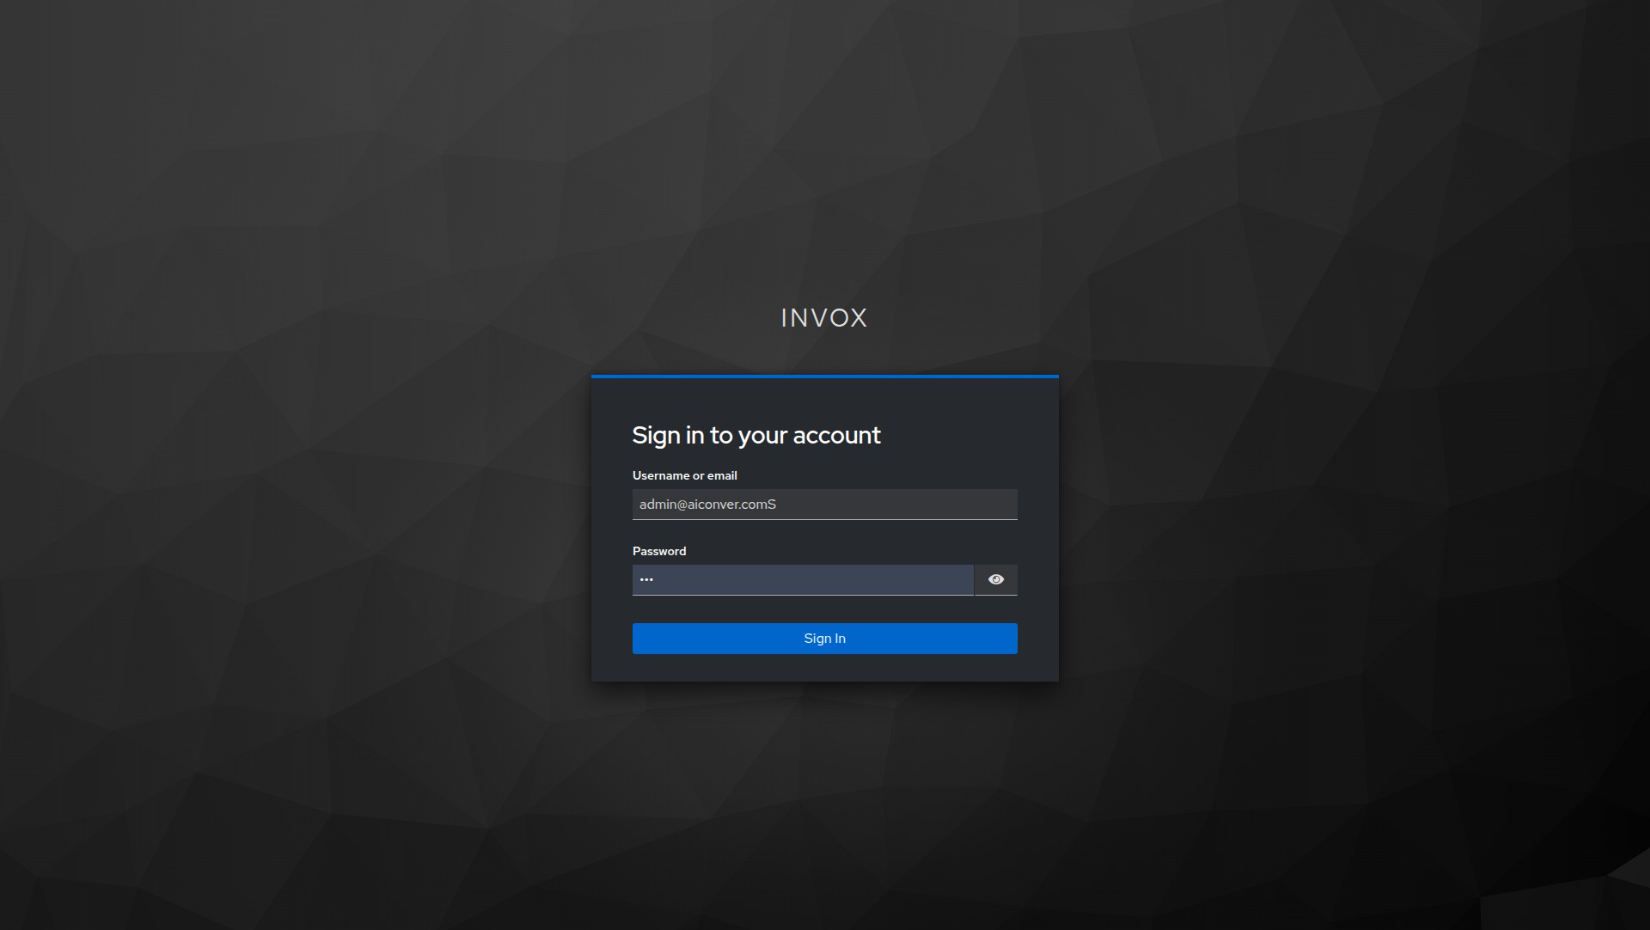
\includegraphics[width=1.0\linewidth]{images/login_interface.png}
  \caption{INVOX authentication interface with Keycloak integration}
  \label{fig:login-interface}
\end{figure}

\subsection{Template Filling Interface}
\label{subsec:ui-template-filling}

\begin{figure}[H]
  \centering
  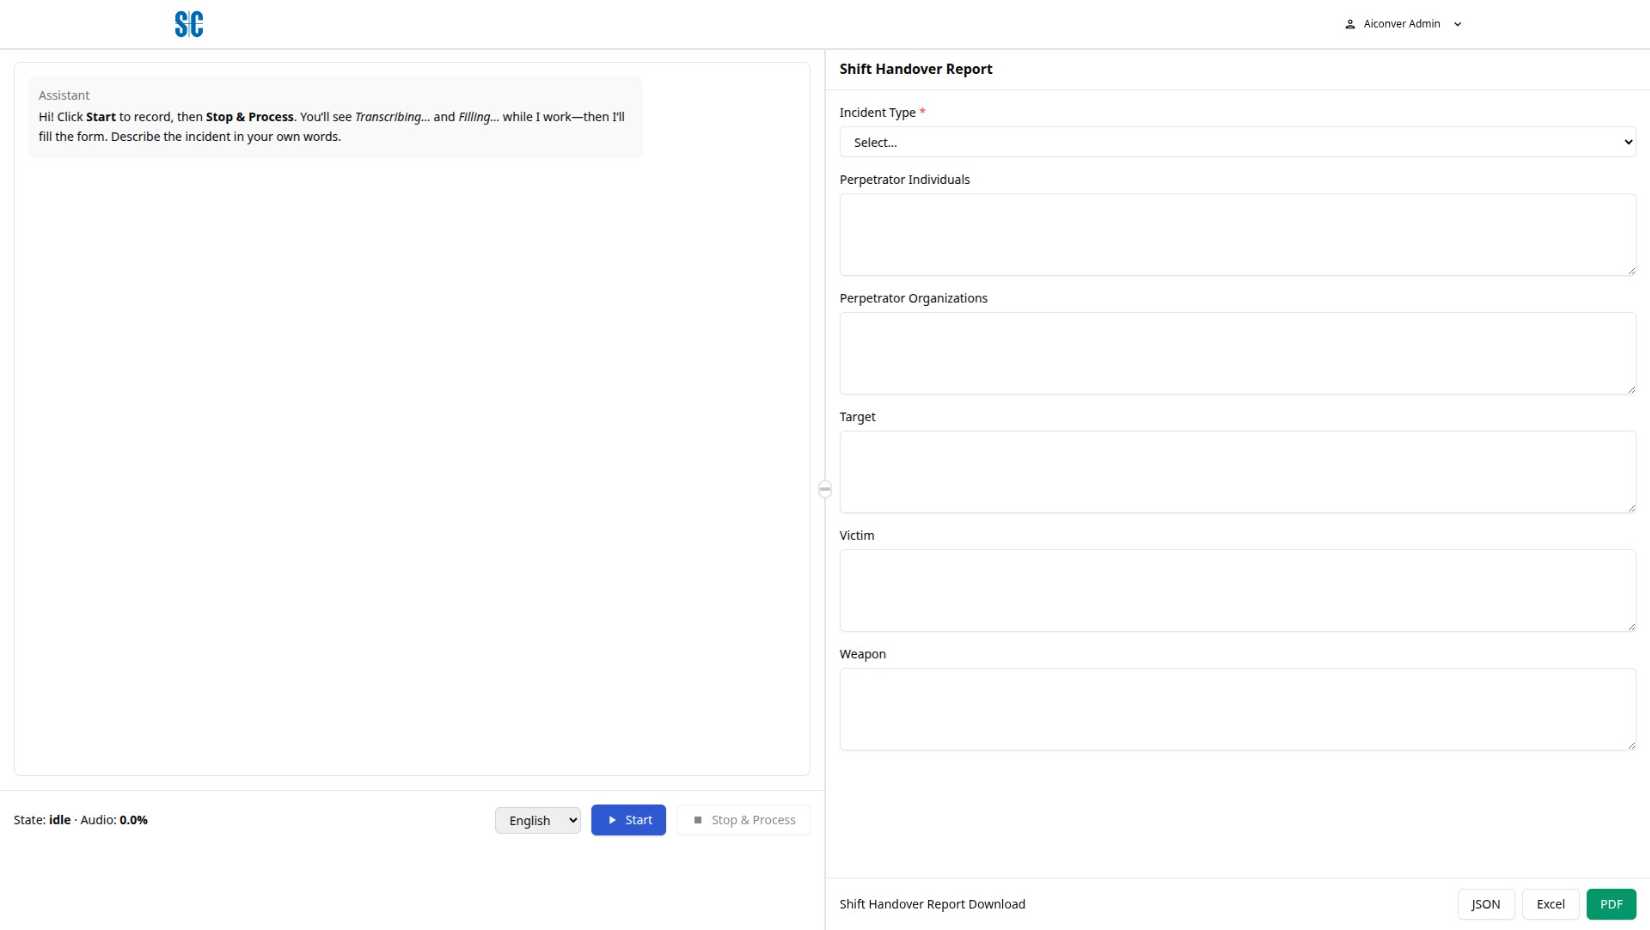
\includegraphics[width=1.0\linewidth]{images/template_interface.png}
  \caption{Template filling interface with voice input (bottom-left), structured form (right), and interactive chat panel}
  \label{fig:template-interface}
\end{figure}

The interface consists of three main components (Figure~\ref{fig:template-interface}): the audio recording panel at the bottom-left, the structured template form on the right, and an interactive chat panel for clarifications.

\subsubsection{Audio Recording Panel}

The recording panel provides a "Start" button to initiate audio capture. During recording, the button changes to "Stop \& Process." When clicked, the system transcribes the audio and extracts template values using the selected strategy. A strategy selector menu allows users to choose between S1, S2, S3, or S4 before processing, enabling them to balance speed versus accuracy based on the template's importance.

\subsubsection{Structured Template Form}

The right side displays the template form with fields organized by category (Incident Type, Perpetrator Information, Target, Victim, Weapon). As the system processes audio input, fields are automatically populated based on the extraction results. Each field type renders appropriately: dropdowns for enumerated values, text areas for descriptions, and specialized inputs for dates and numbers. Fields populated by AI extraction are marked with confidence indicators, with low-confidence fields highlighted to direct user attention.

Users can directly edit any field value, lock fields to prevent overwriting during subsequent recordings, and review the source of each value (AI-extracted versus manually entered). The form validates inputs against schema constraints before allowing submission.

\subsubsection{Interactive Chat Panel}

The chat panel provides real-time feedback during template filling. When the system identifies missing required fields, conflicting information, or ambiguous extractions, it posts messages requesting clarification. For example, if the perpetrator field contains uncertain information, the chat prompts the user to provide more specific details. This interactive guidance reduces iteration cycles by identifying issues immediately rather than after submission.

\subsection{Template Export}

Once users complete template review, the interface provides export options in JSON, Excel, and PDF formats through a download button group. All templates are automatically persisted to PostgreSQL upon processing, ensuring data preservation regardless of export actions.

Having established the complete implementation of the Invox system—from backend agent architecture to frontend user interface—the next chapter evaluates this implementation empirically. Chapter~\ref{chap:evaluation} applies the system to the MUC-4 benchmark and measures its performance against the six requirements (R1–R6) established in Chapter~\ref{sec:requirements}. The evaluation compares the four architectural strategies quantitatively, examining their trade-offs in accuracy, cost, latency, and user satisfaction.